% !TEX program = xelatex
\documentclass[10pt, aspectratio=1610]{beamer}
\usepackage[utf8]{inputenc}
\usetheme{metropolis}
\usepackage{amsmath,listings,lstautogobble,appendixnumberbeamer,booktabs}

\newcommand{\code}[1]{\texttt{\smaller#1}}
\newcommand{\reals}{\mathbb{R}}
\newcommand{\complex}{\mathbb{C}}
\newcommand{\E}{\mathbf{E}}
\newcommand{\var}{\mathrm{Var}}
\newcommand{\cov}{\mathrm{Cov}}

\definecolor{mygreen}{rgb}{0,0.6,0}
\definecolor{mygray}{rgb}{0.5,0.5,0.5}
\definecolor{mymauve}{rgb}{0.58,0,0.82}
\definecolor{bggray}{rgb}{0.95,0.95,0.975}

\lstdefinestyle{prompt}{ %
	backgroundcolor=\color{bggray},
	basicstyle=\ttfamily\footnotesize,
	language=bash,
	frame=none,
	morekeywords={\$},
	keywordstyle=\ttfamily\sl,
	numbers=left,
	numberstyle=\ttfamily\tiny\color{mygray},
	autogobble=true
}

\lstdefinestyle{python_output}{ %
	backgroundcolor=\color{bggray},
	basicstyle=\ttfamily\footnotesize,
	language=bash,
	frame=none,
	keywordstyle=\color{black},
	numbers=left,
	numberstyle=\ttfamily\tiny\color{mygray},
	stringstyle=\color{black},
	autogobble=true
}

\lstset{ %
	backgroundcolor=\color{bggray},   % choose the background color; you must add \usepackage{color} or \usepackage{xcolor}; should come as last argument
	basicstyle=\ttfamily\footnotesize,        % the size of the fonts that are used for the code
	breakatwhitespace=false,         % sets if automatic breaks should only happen at whitespace
	breaklines=true,                 % sets automatic line breaking
	captionpos=b,                    % sets the caption-position to bottom
	commentstyle=\color{mygreen},    % comment style
	deletekeywords={...},            % if you want to delete keywords from the given language
	escapeinside={\%*}{*)},          % if you want to add LaTeX within your code
	extendedchars=true,              % lets you use non-ASCII characters; for 8-bits encodings only, does not work with UTF-8
	frame=none,                      % adds a frame around the code
	keepspaces=true,                 % keeps spaces in text, useful for keeping indentation of code (possibly needs columns=flexible)
	keywordstyle=\color{blue},       % keyword style
	language=Python,                 % the language of the code
	morekeywords={*,True,False,numpy,scipy,matplotlib,np,sc,plt,la,linalg,whos,det,inv,diag,array,allclose,linspace,pyplot,plt,show,subplots,plot,grid,legend,set_xlabel,set_ylabel,set_title,argmax,num,linewidth,color,label,rc,usetex,math,pandas,DataFrame,random,zeros,nanmax,nanargmax,nan,ones,polyfit,polyval,optimize,fsolve,interpolate,interp1d,stats,norm,diff,cdf,pdf,reshape,polynomial,hermite,hermgauss,sqrt,fftpack,as,sparse,spmatrix,jit,njit,cuda,vectorize,guvectorize,stencil,@jit,@njit,@cuda,@vectorize,@guvectorize,@stencil...},       % if you want to add more keywords to the set
	numbers=left,                    % where to put the line-numbers; possible values are (none, left, right)
	numbersep=5pt,                   % how far the line-numbers are from the code
	numberstyle=\ttfamily\tiny\color{mygray}, % the style that is used for the line-numbers
	rulecolor=\color{mygray},         % if not set, the frame-color may be changed on line-breaks within not-black text (e.g. comments (green here))
	showspaces=false,                % show spaces everywhere adding particular underscores; it overrides 'showstringspaces'
	showstringspaces=false,          % underline spaces within strings only
	showtabs=false,                  % show tabs within strings adding particular underscores
	stepnumber=1,                    % the step between two line-numbers. If it's 1, each line will be numbered
	stringstyle=\color{mymauve},     % string literal style
	tabsize=2,						 % sets default tabsize to 2 spaces
	autogobble=true%,	             % adjusts indentation and newline characters
	%title=\lstname                   % show the filename of files included with \lstinputlisting; also try caption instead of title
}


\definecolor{teal}{rgb}{0, 0.53, 0.53}

\hypersetup{colorlinks,linkcolor=,urlcolor=teal}

\setmonofont[Scale=0.9, BoldFont={Fira Mono Medium}]{Fira Mono}
\setbeamercolor{normal text}{bg=white}

\author{Andrea Pasqualini}
\institute{Bocconi University}
\date{March 2020}
\title{High-Performance Computing for Economists}
\subtitle{An Introduction to Numba}

\begin{document}

\maketitle

\begin{frame}
  \frametitle{Outline}

  \tableofcontents

\end{frame}

\section{Introduction}

\begin{frame}
  \frametitle{Why do we need to speed up code?}

  \begin{itemize}
    \item
      Economic problems nowadays get complicated very quickly
      \begin{itemize}
        \item
          It is difficult to keep the no.~of state variables down
        \item
          Frictions and information issues call for complicated nonlinearities
        \item
          More complicated nonlinearities call for denser grids for the state space
      \end{itemize}
    \item
      Solving with VFI is time-consuming
    \item
      Developer time is more valuable than computing time, \ldots
    \item
      \ldots but we cannot afford to wait 3 days for solving once
  \end{itemize}

\end{frame}

\begin{frame}
  \frametitle{Why current, high level languages are not enough?}

  Programming languages like Python, R and Matlab share characteristics that make them slow relative to C, C++, Fortran

  \begin{itemize}
    \item They are interpreted, as opposed to compiled
    \item They are weakly typed, as opposed to strongly typed
    \item They are single-threaded, as opposed to multi-threaded
    \item They operate at a higher abstraction level (i.e., they hide technicalities by making assumptions)
  \end{itemize}

  There are middle-ground solutions (e.g., Julia), but we can address everything with Python

\end{frame}

\begin{frame}
  \frametitle{Acceleration VS Parallelization}

  \textbf{Acceleration}
  \begin{itemize}
    \item Take a function, write it in a lower-level, faster language (e.g., C)
    \item Suitable for all functions frequently used
    \item Might require coding in the more complicated language
  \end{itemize}

  \vfill

  \textbf{Parallelization}
  \begin{itemize}
    \item Take a function, make it run on multiple cores with different data
    \item Suitable for all loops that are not serial in nature
    \item Might require coding in the more complicated language
    \item Requires knowledge of: thread, concurrency, parallelism (VS context switching), synchronous and asynchronous execution
  \end{itemize}

  \vfill
  We can achieve both using one Python module: \textbf{Numba}

\end{frame}

\begin{frame}
  \frametitle{What do we need?}

  For acceleration
  \begin{itemize}
    \item Not much, except for knowledge of performing language
  \end{itemize}

  \vfill
  For parallelization
  \begin{itemize}
    \item Knowledge of performing language
    \item Possibly a GPU
  \end{itemize}

\end{frame}

\begin{frame}
  \frametitle{Useful concepts}

  \small
  \begin{itemize}
    \item Compilers VS interpreters
      \begin{itemize}
        \item Interpreters return the result of a program
        \item Compilers return a program written in machine language (e.g., assembly)
        \item Compiled programs are customized to the specific hardware and run ``closer to the silicon''
      \end{itemize}
    \item Static VS dynamic typing
      \begin{itemize}
        \item Statically typed languages do not try to infer the type of variables: the programmer needs to declare the type, and only then can assign a (compatible) value (e.g., \texttt{int x = 1;})
        \item Weakly typed languages infer the types: the programmer just assigns values to variables, and the language heavy-lifts to infer the types from context (e.g., \texttt{a = 1.2})
      \end{itemize}
    \item Single- VS multi-threading
      \begin{itemize}
        \item Single-threaded tasks run on one core, sequentially
        \item Multi-threaded tasks run on multiple cores, in parallel
        \item Tasks that are independent of each other can be run in parallel
      \end{itemize}
  \end{itemize}

\end{frame}

\begin{frame}
  \frametitle{Useful concepts}

  By choosing a compiled, statically typed language that allows multi-threading, we need to

  \begin{itemize}
    \item Compile the program (remove an abstraction level)
    \item Declare types (make code ``less flexible'')
    \item Design code around tasks (make code modular)
    \item Potentially arrange tasks across threads
  \end{itemize}

  \vfill

  A word on design: the UNIX philosophy might help
  \begin{itemize}
    \item \emph{Write programs that do one thing and do it well}
    \item \emph{Write programs to work together}
  \end{itemize}

\end{frame}

\begin{frame}[fragile]
  \frametitle{Python decorators}

  Python decorators are just \emph{syntax} that alters functions and methods

  \vfill

  These two are equivalent

  \begin{columns}
    \begin{column}{0.4\textwidth}
      \begin{lstlisting}[language=python]
        @staticmethod
        def f(x):
            # something
      \end{lstlisting}
    \end{column}
    \begin{column}{0.4\textwidth}
      \begin{lstlisting}[language=python]
        def f(x):
            # something
        f = staticmethod(f)
      \end{lstlisting}
    \end{column}
  \end{columns}

  \vfill

  Also known as \emph{syntactic sugar}: syntax that only improves readability, without any intrinsic added meaning

\end{frame}

\section{Acceleration}

\begin{frame}
  \frametitle{Acceleration}

  There are two main ways with Python

  \begin{itemize}
    \item \textbf{Cython} (\url{https://cython.org/})
      \begin{itemize}
        \item A native C extension to Python
        \item Write code with Python syntax, but C semantics
        \item Before execution, the Cython function is translated to C code and compiled to machine code (saved on disk)
        \item Requires a C compiler on your computer
      \end{itemize}
    \item \textbf{Numba} (\url{http://numba.pydata.org/})
      \begin{itemize}
        \item An implementation of the LLVM infrastructure
        \item Write Python code and instruct Numba to parse it
        \item During execution, LLVM compiles the function to machine code \emph{just in time} for use (saved on memory)
      \end{itemize}
  \end{itemize}

  Here I will show \alert{Numba}.
  Cython can be faster than Numba if well optimized, but optimization requires a lot of manual work and quite some familiarity with the C language.

\end{frame}

\begin{frame}[fragile]
  \frametitle{Accelerating what?}

  The following do the same thing: accumulate an integer from 0 to a billion

  \begin{columns}[T]
    \begin{column}{0.35\textwidth}
      \texttt{loop.py}
      \begin{lstlisting}[language=python]
        x = 0
        i_max = 1000000000
        for i in range(i_max):
            x += 1
      \end{lstlisting}
    \end{column}
    \begin{column}{0.45\textwidth}
      \texttt{loop.c}
      \begin{lstlisting}[language=c]
        int main () {
            int x = 0;
            int i_max = 1000000000;
            for (int i = 0; i < i_max; i++) {
                x += 1;
            }
        }
      \end{lstlisting}
    \end{column}
  \end{columns}

  Running in the terminal (requires Bash/Zsh)
  \begin{columns}[T]
    \begin{column}{0.35\textwidth}
      \begin{lstlisting}[language=bash]
        $ time python3 ./loop.py
        real    1m41.928s
        user    1m39.734s
        sys     0m0.078s
      \end{lstlisting}
    \end{column}
    \begin{column}{0.45\textwidth}
      \begin{lstlisting}[language=bash]
        $ g++ ./loop.c  # outputs file 'a.out'
        $ time ./a.out
        real    0m1.708s
        user    0m1.688s
        sys     0m0.000s
      \end{lstlisting}
    \end{column}
  \end{columns}

\end{frame}

% \begin{frame}[fragile]
%   \frametitle{Accelerating what?}




% \end{frame}

\begin{frame}[fragile]
  \frametitle{Accelerating with Numba}

  \href{https://numba.pydata.org/numba-doc/latest/user/5minguide.html}{Numba} is a do-it-all module for Python that integrates with NumPy

  \vfill

  In a nutshell
  \begin{itemize}
    \item \href{https://numba.pydata.org/numba-doc/dev/reference/jit-compilation.html#numba.jit}{\texttt{@jit}}: do-it-all
      \begin{itemize}
        \item Compiles the code with LLVM \emph{just-in-time}
      \end{itemize}
    \item \href{https://numba.pydata.org/numba-doc/dev/reference/jit-compilation.html#numba.vectorize}{\texttt{@vectorize}}: write it for scalars, run it on same-size arrays
      \begin{itemize}
        \item Numba wraps the code with efficient \texttt{for} loop for us
        \item Returns a \href{https://docs.scipy.org/doc/numpy/reference/ufuncs.html}{\lstinline{numpy.ufunc}}
      \end{itemize}
    \item \href{https://numba.pydata.org/numba-doc/dev/reference/jit-compilation.html#numba.guvectorize}{\texttt{@guvectorize}}: generalization of \lstinline{@vectorize}
      \begin{itemize}
        \item Allows for passing arrays of different sizes and access elements
        \item The output is passed as input
      \end{itemize}
    \item \href{https://numba.pydata.org/numba-doc/dev/user/stencil.html#numba-stencil}{\texttt{@stencil}}: simplifies writing of stencil patterns
      \begin{itemize}
        \item Write it with relative array indexing
        \item Numba wraps it with appropriate loops
        \item Numba takes care of out-of-bounds exceptions
      \end{itemize}
  \end{itemize}

\end{frame}

\begin{frame}[fragile]
  \frametitle{Numba.jit}

  Compiles the decorated function just-in-time to machine code

  \vfill

  Example
  \begin{lstlisting}[language=python]
    @jit
    def mySum(a, b):
        return a + b
  \end{lstlisting}

  \vfill

  As simple as that?
  Almost\dots

  \vfill

  There is a big performance difference between

  \vspace{1ex}
  \begin{columns}
    \begin{column}{0.45\textwidth}
      \alert{\texttt{nopython}} mode
      \begin{lstlisting}
        @jit(nopython=True)
        def mySum(a, b):
            return a + b
      \end{lstlisting}
    \end{column}
    \begin{column}{0.45\textwidth}
      \alert{\texttt{object}} mode
      \begin{lstlisting}
        @jit(nopython=False)
        def mySum(a, b):
            return a + b
      \end{lstlisting}
    \end{column}
  \end{columns}

\end{frame}

\begin{frame}[fragile]
  \frametitle{Numba.jit: \texttt{nopython} VS \texttt{object} modes}

  \begin{columns}[T]
    \begin{column}{0.45\textwidth}
      \alert{\texttt{nopython}} mode
      \begin{itemize}\small
        \item Default for \lstinline{@jit}
        \item Avoids the Python interpreter when compiling
        \item Cannot deal with stuff Numba does not know about (e.g., Pandas)
        \item Recommended for best performance
      \end{itemize}
    \end{column}
    \begin{column}{0.45\textwidth}
      \alert{\texttt{object}} mode
      \begin{itemize}\small
        \item Fallback option for \lstinline{@jit}
        \item Uses the Python interpreter when compiling
        \item Deals with any Python object
        \item Slower than \texttt{nopython} mode
      \end{itemize}
    \end{column}
  \end{columns}

  \vfill

  Hints
  \begin{itemize}
    \item Write small, modular functions
    \item Optimize everything in \alert{\texttt{nopython}} mode
    \item \lstinline{@njit} is equivalent to \lstinline{@jit(nopython=True)}
    \item Use for not-so-general functions
    \item General speed-ups (e.g., if you have many \texttt{for} loops)
  \end{itemize}

\end{frame}

\begin{frame}[fragile]
  \frametitle{Numba.vectorize}

  Numpy's universal functions, \texttt{ufuncs}, are written as if they were working with scalars, but then you can use them for arrays

  \vfill

  Example
  \begin{lstlisting}[language=python]
    @vectorize(float64(float64, float64))
    def mySum(a, b)
        return  a + b
  \end{lstlisting}

  \vfill

  Bonuses and catches
  \begin{itemize}
    \item No need to pass in the \emph{function signature} (but is recommended)
    \item Numba wraps the function in an efficient loop
    \item The resulting function is a Numpy \texttt{ufunc} (compare with \lstinline{@jit})
      \begin{itemize}
        \item Broadcasting (e.g., sum between $n \times m$ and $n \times 1$ arrays)
        \item Accumulation (e.g., \texttt{np.cumsum})
        \item Reduction (e.g., automatic \texttt{np.squeeze})
      \end{itemize}
  \end{itemize}

\end{frame}

\begin{frame}[fragile]
  \frametitle{Numba.guvectorize}

  Numpy's \texttt{ufuncs} are limited: you cannot arbitrarily mix array sizes (up to broadcasting)

  \vfill

  Example
  \begin{lstlisting}[language=python]
    @guvectorize([(float64[:], float64, float64[:])], '(n), () -> (n)')
    def scalar_multiplication(x, a, result):
        for i in range(x.shape[0]):
            result[i] = a * x[i]
  \end{lstlisting}

  \vfill

  % Need to indicate more structure
  % \begin{itemize}
  %   \item Semantic output is passed as input
  %   \item Need to provide the (list of) function signature(s)
  %   \item Need to provide the \emph{layouts} of inputs
  %     \begin{itemize}
  %       \item Scalars: \lstinline{float64}, \lstinline{'()'}
  %       \item 1D arrays: \lstinline{float64[:]}, \lstinline{'(n)'}
  %       \item 2D arrays: \lstinline{float64[:,:]}, \lstinline{'(n, m)'}
  %     \end{itemize}
  % \end{itemize}

  \begin{columns}
    \begin{column}{0.45\textwidth}
      Need to indicate more structure
      \begin{itemize}\small
        \item Semantic output is passed as input
        \item Need to provide the (list of) function signature(s)
        \item Need to provide the \emph{layouts} of inputs
      \end{itemize}
    \end{column}
    \begin{column}{0.35\textwidth}
      \begin{table}
        \footnotesize
        \begin{tabular}{lll}
          \toprule
          Array & Signature & Layout \\
          \cmidrule{2-3}
          Scalar & \lstinline[]!float64! & \lstinline[]!'()'! \\
          1D array & \lstinline[]!float64[:]! & \lstinline[]!'(n)'! \\
          2D array & \lstinline[]!float64[:,:]! & \lstinline[]!'(n, m)'! \\
          \dots & \dots & \dots \\
          \bottomrule
        \end{tabular}
      \end{table}
    \end{column}
  \end{columns}

\end{frame}

\begin{frame}[fragile]
  \frametitle{Numba.stencil}

  \begin{columns}
    \begin{column}{0.75\textwidth}
      \emph{Stencils} are computational patterns that, for every element of the input array, take elements in a neighborhood and combine them
    \end{column}
    \begin{column}{0.15\textwidth}
      \begin{figure}
        \centering
        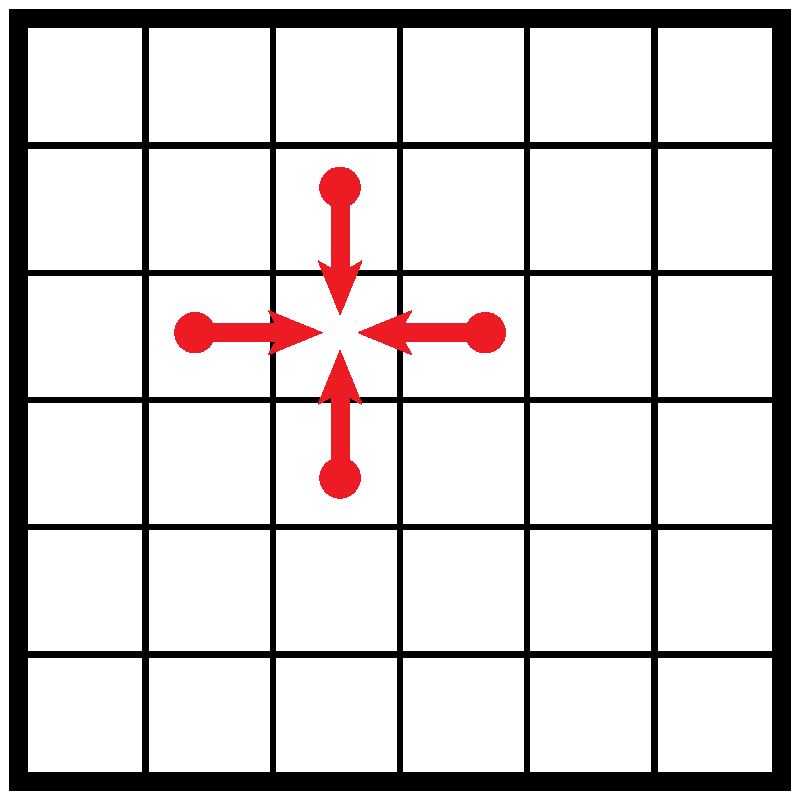
\includegraphics[width=\textwidth]{./img/stencil.pdf}
      \end{figure}
    \end{column}
  \end{columns}

  \vfill

  Example
  \begin{lstlisting}[language=python]
    @stencil
    def moving_average(x):  # stencil kernel
        return 0.10 * x[-2] + 0.25 * x[-1] + 0.30 x[0] + 0.25 * x[1] + 0.10 x[2]
  \end{lstlisting}

  \vfill

  Array indexing is \emph{relative} to each element
  \begin{itemize}
    \item The stencil \emph{kernel} is run for every element $A_{i,j}$
    \item \lstinline{A[h, k]} within kernel actually means \lstinline{A[i + h, j + k]}
    \item Numba takes care of looping across all elements
    \item Numba takes care of handling out-of-bounds exceptions
  \end{itemize}

\end{frame}

\begin{frame}
  \frametitle{Further optimizations}

  \begin{itemize}
    \item \texttt{fastmath}: accelerates purely-mathematical computations
      \begin{itemize}
        \item Available in: \lstinline{@jit}
        \item Refuses to work with \texttt{NaN}'s, \texttt{Inf}'s
        \item Lowers precision of floating-point calculations
      \end{itemize}
    \vfill
    \item \texttt{target}: allows for specialized hardware deployment
      \begin{itemize}
        \item Available in: \lstinline{@vectorize} and \lstinline{@guvectorize}
        % \item Allows \lstinline{'cpu'}, \lstinline{'parallel'} and \lstinline{'cuda'}
        % \item \lstinline{'parallel'} and \lstinline{'cuda'} require specification of function signature
        \item \lstinline{target='cpu'} (default) runs code on CPU, in single-threaded mode
        \item \lstinline{target='parallel'} automatically uses all threads on CPU (requires function signature)
        \item \lstinline{target='cuda'} automatically uses an Nvidia GPU, if available (requires function signature)
      \end{itemize}
    \vfill
    \item \texttt{cache}: saves compiled version on disk
      \begin{itemize}
        \item Available in: \lstinline{@jit}, \lstinline{@vectorize} and \lstinline{@guvectorize}
        \item LLVM compilation saves compiled code to RAM by default
        \item \lstinline{cache=True} saves compiled code on disk, for easy reuse
        \item Incompatible with \lstinline{target='cuda'}
      \end{itemize}
  \end{itemize}

\end{frame}

\section{Parallelization}

\begin{frame}
  \frametitle{Parallelization}

  Anything that has more than one computing core supports parallelization

  \begin{itemize}
    \item CPUs nowadays are all multi-core and often support hyper-threading (i.e., one core executes two threads)
    \item GPUs have many more cores than CPUs, but run at lower clock frequencies
    \item There are many models of parallelization: here we look at \emph{SIMD} (Same Instruction, Multiple Data)
  \end{itemize}

  Here I show how to parallelize on \alert{GPU}s.
  Parallelizing on CPUs is similar in the concepts, and easy to do with Numba.

\end{frame}

\begin{frame}
  \frametitle{Why can GPUs help?}

    GPUs are typically employed in videogames
    \begin{itemize}
      \item
        Games graphics are typically vector graphics that need to be displayed on screen
      \item
        Screens are 2D grids of pixels and the graphics card is in charge of deciding what color each pixel should show
      \item
        Problem: ``smooth'' gaming performance requires the computer to refresh the screen at a rate of at least 60 frames per second
      \item
        The graphics card needs to process data from the CPU, compute all algebraic operations imposed by simulated movement (e.g., turning around in a game) and return the colors that the array of pixels should display
      \item
        Take-away: graphics cards are optimized to run \emph{many} linear algebra operations with floating point numbers in parallel
    \end{itemize}

\end{frame}

\begin{frame}
  \frametitle{Why can GPUs help? A graphical illustration}

  % In graphics applications, GPUs solve a bunch of projection problems

  \begin{columns}
    \begin{column}{0.4\textwidth}
      In graphics applications, GPUs solve a bunch of projection problems
    \end{column}
    \begin{column}{0.5\textwidth}
      \begin{figure}
        \centering
        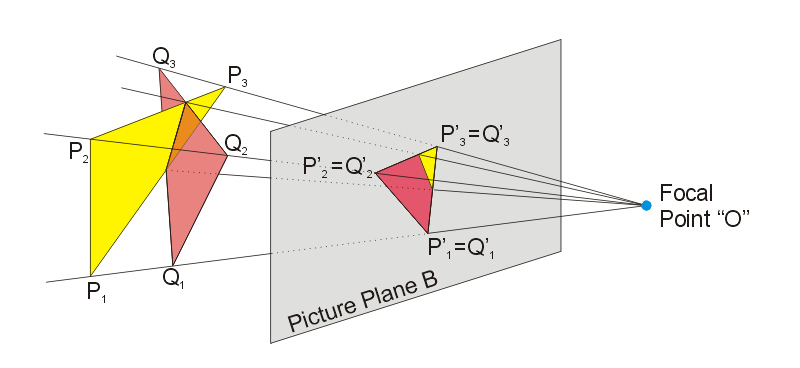
\includegraphics[width=\textwidth]{./img/Perspective_Projection_Principle.jpg}
      \end{figure}
    \end{column}
  \end{columns}

  \begin{itemize}
    \item Desired graphic is projected onto a plane (the screen) with a set of polygons (typically, triangles)
    \item Movements in graphic are projected to shifts/rotations of polygon vertices
  \end{itemize}

  Again: GPUs are optimized to execute a ton of linear algebra operations in parallel

\end{frame}

\begin{frame}
  \frametitle{Why do we not use GPUs for everything?}

  Because they are specialized hardware, GPUs are bad for...%
    \footnote{
      \url{https://cs.stackexchange.com/questions/121080/}
    }

  \begin{itemize}
    \item
      Everything that needs to run in serial (e.g., \texttt{for} loops that run in serial)
    \item
      Everything that requires \emph{large} amounts of RAM
    \item
      Everything that requires parallel threads to transfer information with each other during execution
    \item
      I/O operations
    \item
      Others...
  \end{itemize}

\end{frame}

\begin{frame}
  \frametitle{How can we use GPUs?}

  First, a few basic concepts

  \begin{itemize}
    \item Design
    \item Hardware
    \item Terminology
    \item Tools
  \end{itemize}

\end{frame}

\begin{frame}
  \frametitle{Code design}

  We cannot expect to just add a decorator to a Python function (as instead would be the case with \texttt{numba.jit})

  \begin{itemize}
    \item Each computing core in the GPU can only deal with simple scalars and simple functions
    \item Parallelizing instructions requires us to decide how to do it
    \item We need to dive into a lower abstraction layer, getting more familiar with the hardware
    \item Depending on the application, GPU execution might add bottlenecks we might have never seen before
  \end{itemize}

  In short, we need to get our hands dirty

\end{frame}

\begin{frame}
  \frametitle{GPU hardware}

  A GPU is a system composed of

  \begin{itemize}
    \item Multi-core processor
      \begin{itemize}
        \item Core: one execution unit
        \item Streaming multiprocessor (SM): a set of cores
        \item GPU unit: a set of SMs
      \end{itemize}
    \item (V-)RAM module
      \begin{itemize}
        \item Smaller RAM capacities than normal RAM
        \item Much faster than normal RAM
      \end{itemize}
    \item PCI-e interface
      \begin{itemize}
        \item Used to communicate with the rest of the computer
        \item Is subject to physical bandwidth limits
      \end{itemize}
    \item Power supply connector
      \begin{itemize}
        \item Delivers supply to the GPU (the GPU might be the most power-hungry component of a computer)
      \end{itemize}
    \item Other components
    \begin{itemize}
      \item e.g., video decoders
      \item e.g., display interface (i.e., circuitry and cables to screens)
    \end{itemize}
  \end{itemize}

\end{frame}

\begin{frame}
  \frametitle{GPU hardware: example}

  Nvidia RTX 2080Ti%
    \footnote{
      \url{https://www.nvidia.com/en-us/geforce/graphics-cards/rtx-2080-ti/}
    }

  \begin{columns}
    \begin{column}{0.6\textwidth}
      \begin{itemize}
        \item Multi-core processor
          \begin{itemize}
            \item No.~of CUDA cores: 4352
            \item Core base frequency: 1350 MHz
          \end{itemize}
        \item VRAM module
          \begin{itemize}
            \item 11 GB
            \item GDDR6: 14 Gbps
            \item Bandwidth 616 GB/s
          \end{itemize}
        \item Misc
          \begin{itemize}
            \item Draws up to 250 W of power
            \item Sustains up to 89°C
            \item MSRP 1199 USD
            \item Blower style air cooling
          \end{itemize}
      \end{itemize}
    \end{column}
    \begin{column}{0.35\textwidth}
      \begin{figure}
        \centering
        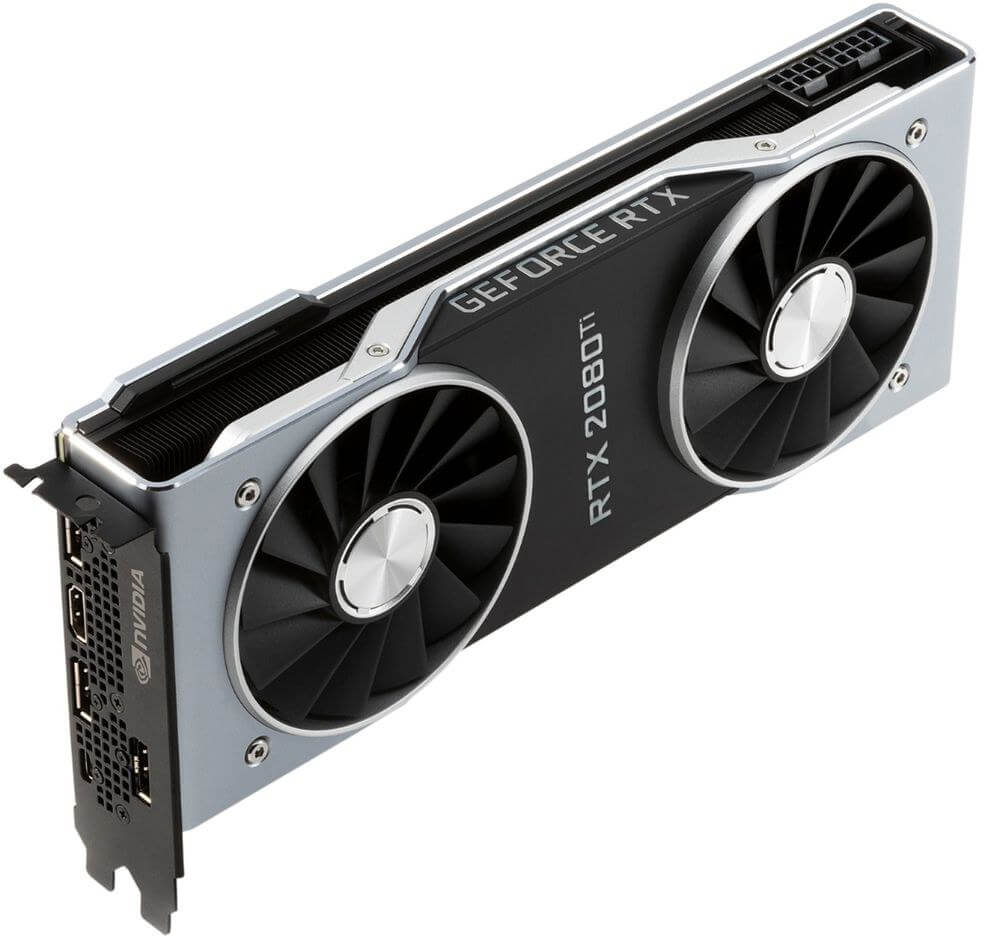
\includegraphics[width=\textwidth]{./img/nvidia-rtx-2080-ti.jpg}
      \end{figure}
    \end{column}
  \end{columns}

\end{frame}

\begin{frame}[fragile]
  \frametitle{Tools}

  The leading hardware vendor for GPU computing is Nvidia%
    \footnote{
      AMD and Intel are in the game, too, but do not really compete over GPGPU
    }

  \begin{itemize}
    \item Nvidia develops CUDA, its own C++-like programming language
    \item Numba has a CUDA module, so we can use Python to do GPU computing
  \end{itemize}

  \vfill
  To install all we need in Python, run in terminal
  \begin{lstlisting}[language=bash]
    conda install cudatoolkit
  \end{lstlisting}

  The version of \texttt{cudatoolkit} you need depends on the hardware you have: older hardware requires older version of \texttt{cudatoolkit}

\end{frame}

\begin{frame}
  \frametitle{Terminology}

  \begin{description}
    \item[Host] The machine orchestrating the hardware (i.e., the CPU)
    \item[Device] The GPU unit
    \item[Kernel] The function that is deployed to the GPU for execution
    \item[Grid] A set of blocks (can organize in arrays, up-to-3D)
    \item[Block] A set of threads (can organize in arrays, up-to-3D)
    \item[Thread] The software counterpart of a processor core, i.e., a queue of instructions to execute
  \end{description}

\end{frame}

\begin{frame}
  \frametitle{Relationship between hardware and software}

  \begin{figure}
    \centering
    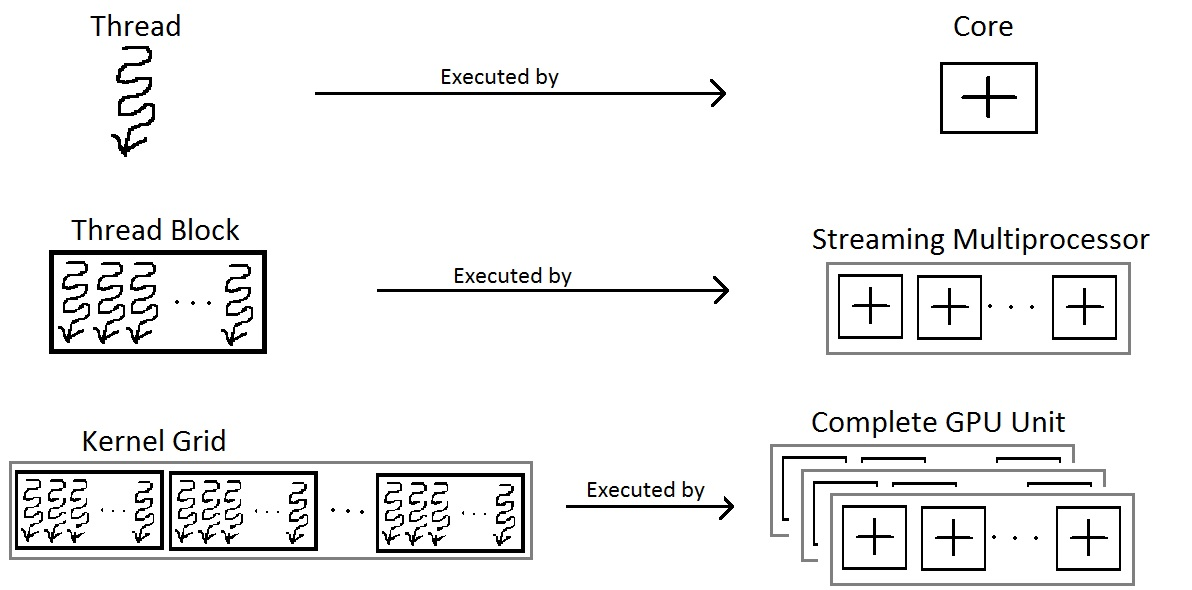
\includegraphics[width=0.7\textwidth, height=0.8\textheight, keepaspectratio]{./img/hw-sw-thread_block.jpg}
  \end{figure}

\end{frame}

\begin{frame}
  \frametitle{Managing threads and blocks}

  \begin{itemize}
    \item The semantics of grouping threads into blocks is up to the user
    \item If done carefully, it allows for big performance
    \item Each core has access to special variables \texttt{blockIdx}, \texttt{blockDim} and \texttt{threadIdx}, with attributes \texttt{x}, \texttt{y} and \texttt{z}
      \begin{itemize}
        \item \texttt{blockIdx} contains the coordinates of the block within the grid
        \item \texttt{blockDim} contains the layout of threads inside the block
        \item \texttt{threadIdx} contains the coordinates of the thread within the block
      \end{itemize}
    \item Given SIMD paradigm, we should balance the workload uniformly across blocks and threads (i.e., do not overload one block and keep another empty)

    \vfill

    \item Example: with VFI, assign each value of the state space to one thread, maximize $V(\cdot)$ at that point within same thread
  \end{itemize}

\end{frame}

\begin{frame}
  \frametitle{Managing threads and blocks: example}

  \begin{columns}
    \begin{column}{0.7\textwidth}
      \begin{itemize}
        \item Grid has dimension $2 \times 3$
        \item \textbf{Block(1, 1)} has \lstinline{blockIdx.x = 1} and \lstinline{blockIdx.y = 1}
        \item \textbf{Block(1, 1)} has \lstinline{blockDim.x = 3} and \lstinline{blockDim.y = 4}
        \item \textbf{Thread(3, 2)} has \lstinline{threadIdx.x = 3} and \lstinline{threadIdx.y = 2}
      \end{itemize}
    \end{column}
    \begin{column}{0.25\textwidth}
      \begin{figure}
        \centering
        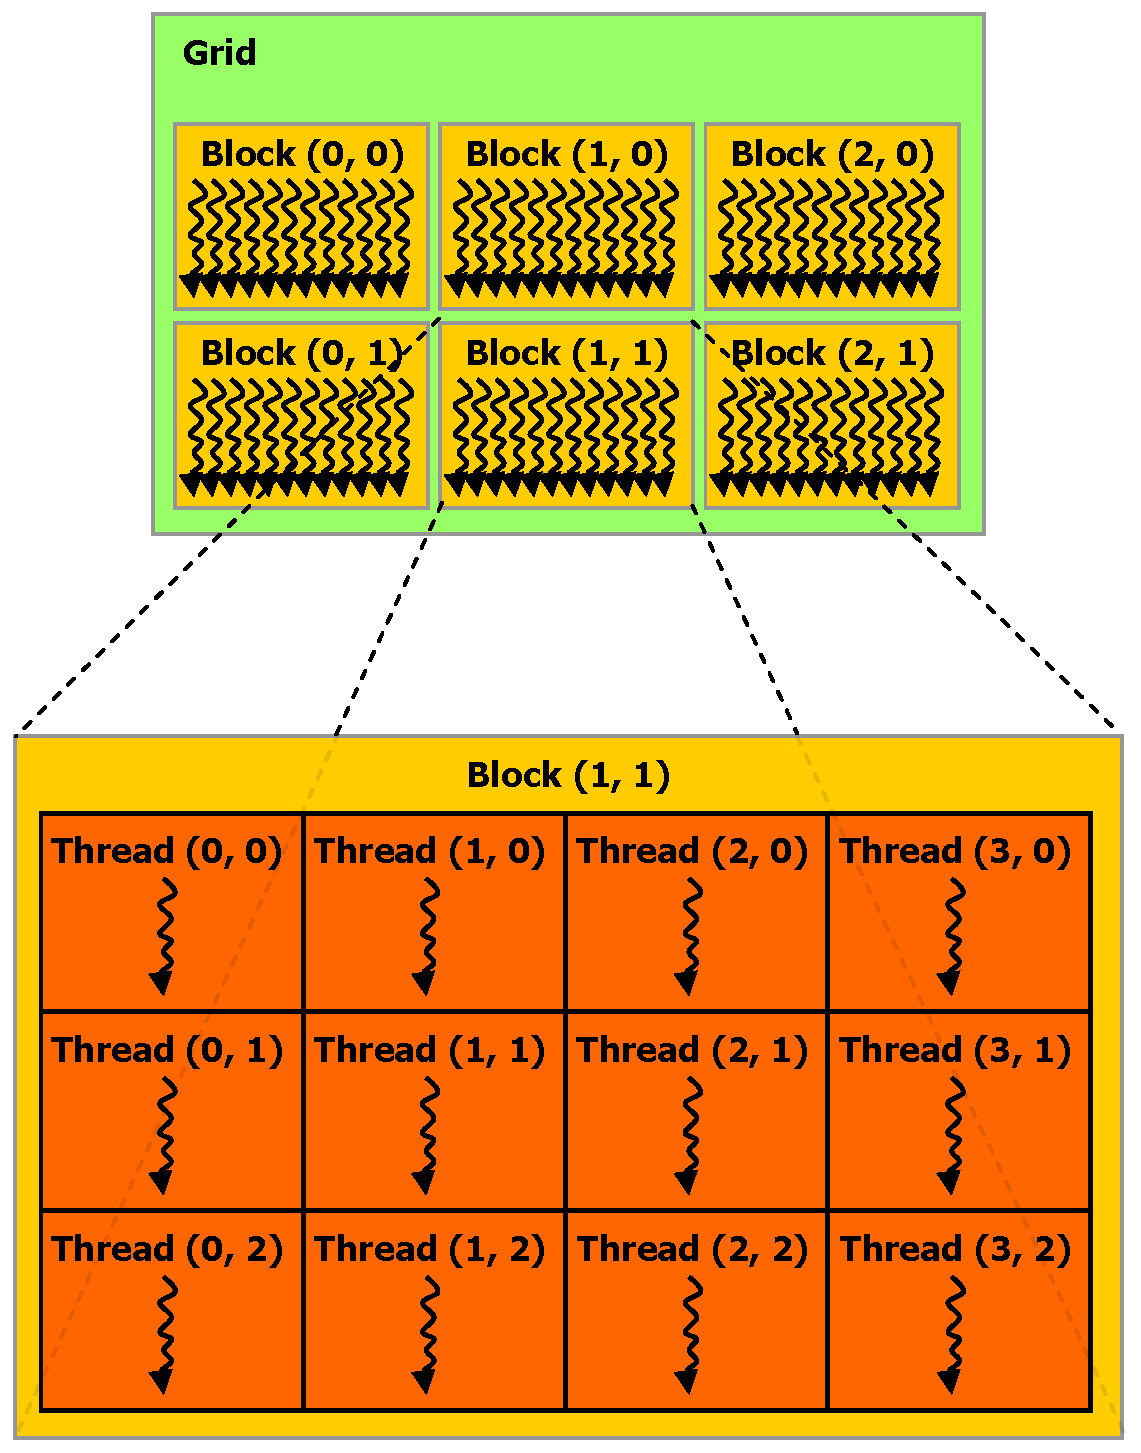
\includegraphics[width=\textwidth, height=0.8\textheight, keepaspectratio]{./img/block-thread.pdf}
      \end{figure}
    \end{column}
  \end{columns}

\end{frame}

\begin{frame}[fragile]
  \frametitle{An example with CUDA}

  This CUDA code parallelizes the sum of two vectors across threads

  \begin{lstlisting}[language=C]
    void vecAddKernel (float *A , float *B , float *C , int n) {
        int index = blockIdx.x * blockDim.x + threadIdx.x;
        if (index < n) {
            C[index] = A[index] + B[index];
        }
    }
  \end{lstlisting}

  \vfill

  What are we looking at?
  \begin{itemize}
    \item \texttt{void} means that the function does not return anything
    \item \texttt{float} and \texttt{int} declare the type of each variable
    \item The semantic output \texttt{C} is passed as an input
    \item \texttt{blockIdx}, \texttt{blockDim} and \texttt{threadIdx} are special CUDA variables to identify the core executing the function
    \item Each core only operates on scalars
  \end{itemize}

\end{frame}

\begin{frame}[fragile]
  \frametitle{An example with CUDA}

  This CUDA code parallelizes the sum of two vectors across threads

  \begin{lstlisting}[language=C]
    void vecAddKernel (float *A , float *B , float *C , int n) {
        int index = blockIdx.x * blockDim.x + threadIdx.x;
        if (index < n) {
            C[index] = A[index] + B[index];
        }
    }
  \end{lstlisting}

  \vfill

  What is happening?
  \begin{itemize}
    \item The host transfers arrays \texttt{A}, \texttt{B} and \texttt{C} to the device memory
    \item Each core is assigned a thread
    \item Each core is aware of \texttt{blockIdx}, \texttt{blockDim} and \texttt{threadIdx}
    \item Cores simultaneously compute the sum $A_i + B_i$ and allocate the result $C_i$ in the right place
    \item Once done, the device returns \texttt{A}, \texttt{B} and \texttt{C} to the host
  \end{itemize}

\end{frame}

\begin{frame}[fragile]
  \frametitle{Numba.cuda}

  \href{https://numba.pydata.org/numba-doc/dev/cuda/index.html}{Numba.cuda} allows for Python code to be compiled into CUDA code

  \vfill

  \begin{lstlisting}[language=python]
    from numba import cuda, void, float64

    @cuda.jit(void(float64[:], float64[:], float64[:]))
    def sum_cuda(a, b, result):
        i = cuda.blockIdx.x * cuda.blockDim.x + cuda.threadIdx.x
        if i < a.shape[0]:
            c[i] = a[i] + b[i]

    n = 640
    a, b, c = np.ones((n,)), np.ones((n,)), np.zeros((n,))
    threads_per_block = 32
    blocks = - (-n // threads_per_block)   # ceil division
    sum_cuda[(blocks, ), (threads_per_block, )](a, b, c)
  \end{lstlisting}

  \vfill

  \begin{itemize}
    \item Calling CUDA kernel requires syntax \lstinline{fun[grid_layout, block_layout](**args)}
    \item Managing blocks and threads is done outside kernel definition
    \item 640 scalar sums happen altogether: this is impossible on a CPU
  \end{itemize}

\end{frame}

\begin{frame}
  \frametitle{GPU parallel might be slower than CPU parallel}

  \begin{itemize}
    \item A big drawback for GPUs is data transfers
      \begin{itemize}
        \item The CPU sends data to GPU
        \item GPU performs computations
        \item GPU returns new data to CPU
      \end{itemize}
    \item These transfers might be a huge bottleneck
    \item Solution
      \begin{itemize}
        \item Small scale problems run faster on CPU
        \item Large scale problems run faster on GPU
        \item Need to experiment with your hardware to find switching point
      \end{itemize}
  \end{itemize}

\end{frame}

\section{VFI benchmarks}

\begin{frame}
  \frametitle{VFI on a GPU}

  Can we parallelize Value Function Iteration?
  \alert{Yes!}

  \begin{itemize}
    \item Maximizing $V(\cdot)$ at each gridpoint of the state space is independent from $V(\cdot)$ at other gridpoints
  \end{itemize}

  \vfill

  Consider the following problem
  \begin{align*}
    V(b) = \max_{c, b'} &\; \log(c) + \beta V(b') \\
    \text{s.t.} &\; c + b' = y + (1+r) b
  \end{align*}

\end{frame}

\begin{frame}[fragile]
  \frametitle{VFI on a GPU: example}

  \begin{lstlisting}[language=python]
    @cuda.jit(void(float64[:], float64[:], float64, float64, float64))
    def vmax_cuda(V, b_grid, r, y, beta):
        ix = cuda.blockIdx.x * cuda.blockDim.x + cuda.threadIdx.x
        VV = pwr(-10.0, 5)
        for ixp in range(b_grid.size):
            cons = (1 + r) * b_grid[ix] + y - b_grid[ixp]
            if cons <= 0:
                period_util = pwr(-10, 5)
            else:
                period_util = log(cons)
            expected = V[ixp]
            values = period_util + beta * expected
            if values > VV:
                VV = values
        V[ix] = VV
  \end{lstlisting}

  \begin{itemize}
    \item The argument of \texttt{\@cuda.jit} is the \emph{function signature}
    \item There is no explicit \texttt{max}, but \texttt{VV} will eventually be the max
    \item Each GPU core computes $V(b)$ at one given gridpoint $b$
  \end{itemize}

\end{frame}

\begin{frame}
  \frametitle{Benchmarks: Hardware test bench}

  An old laptop with discrete graphics: ASUS N550JK ``VivoBook Pro''

  \begin{itemize}
    \item Processor: Intel Core i7-4700HQ
      \begin{itemize}
        \item 4 cores, 8 threads
        \item Base clock frequency: 2.4 GHz
        \item Boost clock frequency: up to 3.4 GHz
      \end{itemize}
    \item RAM: 8 GB DDR3L
    \item GPU: Nvidia GTX 850M (640 CUDA cores @ 936 MHz each)
    \item OS: Ubuntu 19.10 (Linux kernel version 5.3.0)
    \item Price: 899 EUR (in Oct 2014)
  \end{itemize}

\end{frame}

\begin{frame}
  \frametitle{Benchmarks: Methodology}

  \begin{itemize}
    \item Solve the following ($r=1\%$, $\beta=0.95$, $y=1$, $\text{tol}=10^{-4}$)
      \begin{align*}
        V(b) = \max_{c, b'} &\; \log(c) + \beta V(b') \\
        \text{s.t.} &\; c + b' = y + (1+r) b
      \end{align*}

    \vfill
    \item Three functions implementing VFI
      \begin{itemize}
        \item Unoptimized Python function on CPU
        \item Jit-optimized Python function on CPU
        \item CUDA/jit-optimized Python function on GPU
      \end{itemize}
    \item Run each function $N$ times for different values of $n_b$
    \item Compute statistics
    % \item First observation from jit-optimized code discarded
      % \begin{itemize}
        % \item LLVM compilation and CUDA code deployment require time that cannot be attributed to VFI actually running
      % \end{itemize}
  \end{itemize}

\end{frame}

\begin{frame}
  \frametitle{Benchmarks: Results}

  \begin{figure}
    \centering
    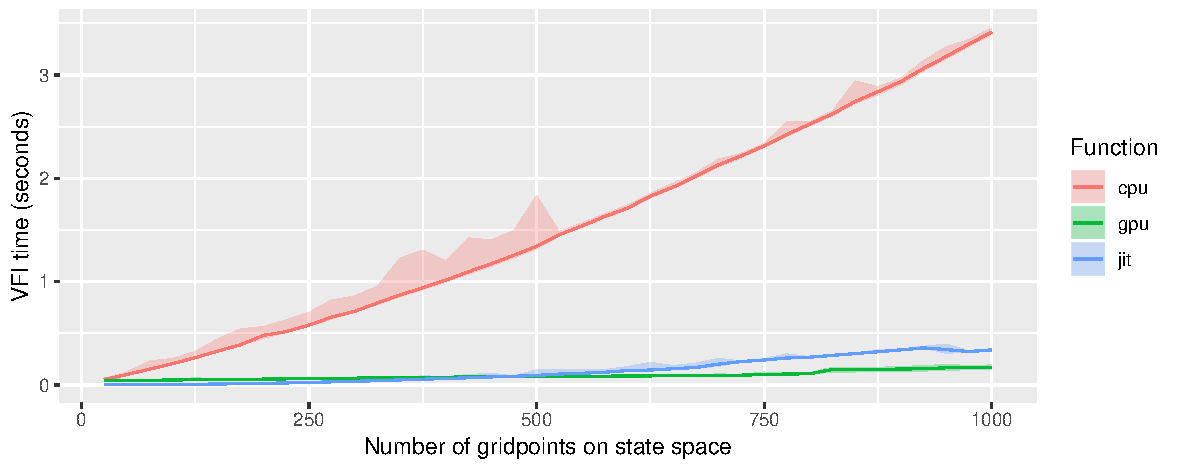
\includegraphics[width=\textwidth, height=0.65\textheight, keepaspectratio]{./img/benchmarks.pdf}
    \caption{\scriptsize
      Averages and min/max ranges of computation times.
      Replications: $N = 1000$.
      Gridpoints on state space: $n_b \in \{ 25, 50, 75, \ldots, 1000 \}$.
      Solid lines are averages.
      Shaded areas are min/max ranges.
    }
  \end{figure}

\end{frame}

\begin{frame}
  \frametitle{Benchmarks: Results (same, in log scale)}

  \begin{figure}
    \centering
    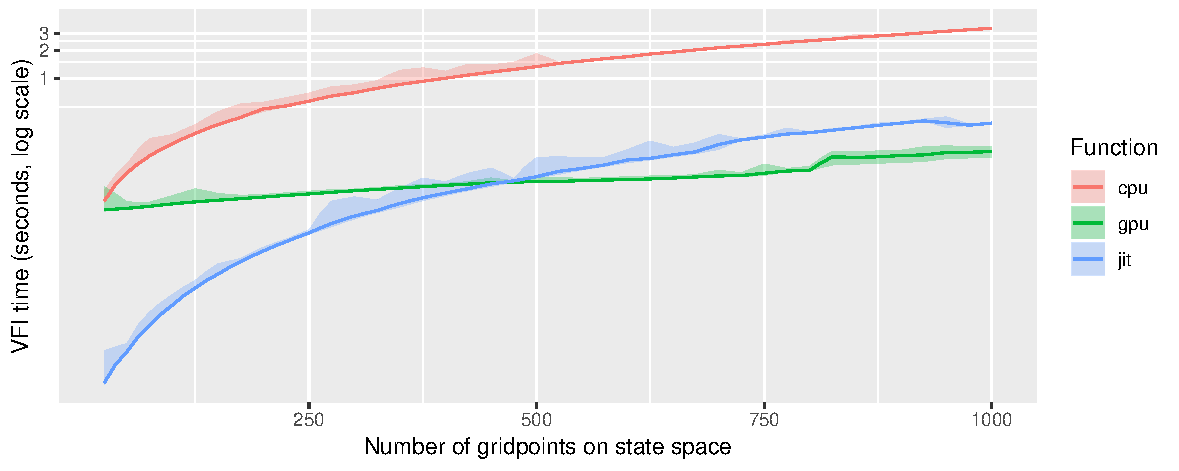
\includegraphics[width=\textwidth, height=0.65\textheight, keepaspectratio]{./img/benchmarks-logscale.pdf}
    \caption{\scriptsize
      Averages and min/max ranges of computation times.
      Replications: $N = 1000$.
      Gridpoints on state space: $n_b \in \{ 25, 50, 75, \ldots, 1000 \}$.
      Solid lines are averages.
      Shaded areas are min/max ranges.
      Vertical axis in log-scale.
    }
  \end{figure}

\end{frame}

\begin{frame}
  \frametitle{Benchmarks: Results, why GPU grows (kinda) linearly}

  Each bar is a block, each square in a block is a thread

  \begin{figure}
    \centering
    \includegraphics<1>[width=\textwidth, height=0.8\textheight, keepaspectratio]{./img/gpu_parallel_visual_1.pdf}%
    \includegraphics<2>[width=\textwidth, height=0.8\textheight, keepaspectratio]{./img/gpu_parallel_visual_2.pdf}%
    \includegraphics<3>[width=\textwidth, height=0.8\textheight, keepaspectratio]{./img/gpu_parallel_visual_3.pdf}%
    \includegraphics<4>[width=\textwidth, height=0.8\textheight, keepaspectratio]{./img/gpu_parallel_visual_4.pdf}%
    \includegraphics<5>[width=\textwidth, height=0.8\textheight, keepaspectratio]{./img/gpu_parallel_visual_5.pdf}%
    % \includegraphics<6>[width=\textwidth, height=0.8\textheight, keepaspectratio]{./img/gpu_parallel_visual_6.pdf}%
    % \includegraphics<7>[width=\textwidth, height=0.8\textheight, keepaspectratio]{./img/gpu_parallel_visual_7.pdf}%
    % \includegraphics<8>[width=\textwidth, height=0.8\textheight, keepaspectratio]{./img/gpu_parallel_visual_8.pdf}%
    % \includegraphics<9>[width=\textwidth, height=0.8\textheight, keepaspectratio]{./img/gpu_parallel_visual_9.pdf}%
    % \includegraphics<10>[width=\textwidth, height=0.8\textheight, keepaspectratio]{./img/gpu_parallel_visual_10.pdf}%
  \end{figure}

\end{frame}

\begin{frame}
  \frametitle{What to parallelize?}

  Suppose your code has two parallelizable steps:
  \begin{itemize}
    \item VFI to solve for the Bellman Equation
    \item Zero-finding routine to solve for equilibrium prices
  \end{itemize}

  What do we parallelize?
  \begin{itemize}
    \item It depends
    \item Try what is faster
    \item Try to match available cores to dimensions of the problem
  \end{itemize}

\end{frame}

\section{Conclusion}

\begin{frame}
  \frametitle{Final remarks}

  \begin{itemize}
    \item HPC is niche in Economics
    \item ``Structural'' people started using it
    \item Strongly consider accelerating code before spending money on hardware

    \vfill

    \item GPU buying considerations
      \begin{itemize}
        \item Custom-built desktop PCs are generally cheaper than equi-potent laptops with discrete graphics cards
        \item Not necessary to buy top-of-the-line, bleeding-edge hardware
        \item What matters is core counts and clock speeds
        \item GPUs one or two generations old are still good for us
        \item GPUs last over time: think of future-proofing
        \item GPU prices slowly decreasing after crypto-currency ``gold rush''
        \item External GPU enclosures are an option, if you don't want to buy a whole new computer and have a laptop with a Thunderbolt 3 port
      \end{itemize}
  \end{itemize}

\end{frame}

\begin{frame}
  \frametitle{Final remarks}

  \begin{itemize}
    \item Optimizing code right off the bat does not help
      \begin{itemize}
        \item First, write your code almost as a brainstorming exercise
        \item Then, \textbf{profile your code} to identify bottlenecks
        \item Finally, optimize code
      \end{itemize}
    \item A serious IDE might help (e.g., \href{https://www.jetbrains.com/pycharm/}{PyCharm})
    \item \href{https://numba.pydata.org/numba-doc/dev/user/index.html}{Numba's user guide} is a gold mine of advice
  \end{itemize}

  \vfill

  \begin{flushright}
    \begin{quotation}
      \hfill``Premature optimization is the root of all evil.''
    \end{quotation}
    --- Donald E.~Knuth
  \end{flushright}

\end{frame}

% \appendix

% \begin{frame}
%   \frametitle{References}

%   \nocite{Numba2015}
%   \bibliographystyle{apalike}
%   \bibliography{references}

% \end{frame}

\end{document}
